
%(BEGIN_QUESTION)
% Copyright 2011, Tony R. Kuphaldt, released under the Creative Commons Attribution License (v 1.0)
% This means you may do almost anything with this work of mine, so long as you give me proper credit

Fire magnetventilstyrte block-ventiler brukes som sikkerhetsavstengning i en petroleumrørledning.  Alle får signal samtidig fra én ``logic solver''-kontroller.  Pålitelighetsverdien ($R$) for hver block-ventil -- sannsynligheten for å følge signalet korrekt -- er vist i diagrammet:

$$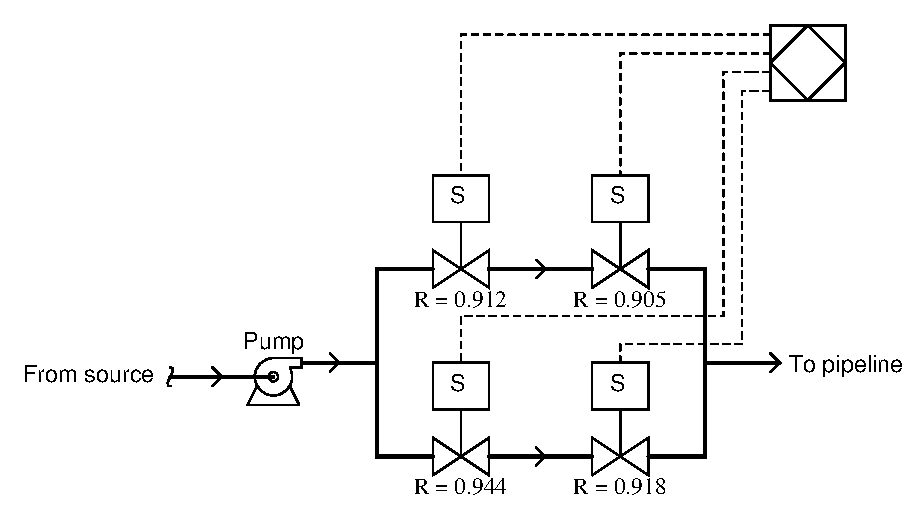
\includegraphics[width=15.5cm]{i00218x01.eps}$$

Bestem \textit{MooN}-klassifiseringene for dette fireventilsystemet, både fra perspektivet \textit{dependability} (evne til å garantere avstengt rørledning) og \textit{security} (evne til å garantere flyt i rørledningen).

\vskip 10pt

MooN (dependability) = \underbar{\hskip 50pt}  \hskip 70pt MooN (security) = \underbar{\hskip 50pt}

\vskip 50pt

Beregn deretter total pålitelighet for at dette fireventilssystemet faktisk kan garantere avstengning, basert på de individuelle pålitelighetene:

\vskip 10pt

$R_{shutoff}$ = \underbar{\hskip 50pt}

\underbar{file i00218}
%(END_QUESTION)





%(BEGIN_ANSWER)

{\it 2 poeng for hvert MooN-svar, pluss 6 poeng for pålitelighetsberegningen}

\vskip 10pt

MooN (dependability) = \underbar{\bf 3oo4}  \hskip 70pt MooN (security) = \underbar{\bf 3oo4}

\vskip 10pt

$R_{shutoff}$ = \underbar{\bf 0.98709}

%(END_ANSWER)





%(BEGIN_NOTES)

{\bf This question is intended for exams only and not worksheets!}

%(END_NOTES)

